\documentclass[10pt, svgnames, compress, red]{beamer}
\usepackage{lmodern}
\usepackage{palatino}
\usepackage[T1]{fontenc}
\usepackage[utf8]{inputenc}
\usepackage[french]{babel}

%%%%%%%%%%%%%%%%%%%%%%%%%%%%%%%%%%%%%%%%%%%%%%%%%%%%%%%%%%%%%%%%%%%%%%%%%%%%%%%%%%%%%%%%%%%%%%%%%%%%%%%%%%%%%%
% PACKAGES
%%%%%%%%%%%%%%%%%%%%%%%%%%%%%%%%%%%%%%%%%%%%%%%%%%%%%%%%%%%%%%%%%%%%%%%%%%%%%%%%%%%%%%%%%%%%%%%%%%%%%%%%%%%%%%

%\usepackage{multimedia}				% to use multimedia
\usepackage{graphicx}				  % to use graphics
\usepackage{subfigure}				% to use figure in figure
\hypersetup{pdfstartview={Fit}}
\graphicspath{{./images/}}		% to say where are image
\usepackage{natbib}
\usepackage{caption}
\usepackage{appendixnumberbeamer}
% \RequirePackage{pageGardeEnsta}
% \usepackage[svgnames]{xcolor}

%%%%%%%%%%%%%%%%%%%%%%%%%%%%%%%%%%%%%%%%%%%%%%%%%%%%%%%%%%%%%%%%%%%%%%%%%%%%%%%%%%%%%%%%%%%%%%%%%%%%%%%%%%%%%%
% THEME
%%%%%%%%%%%%%%%%%%%%%%%%%%%%%%%%%%%%%%%%%%%%%%%%%%%%%%%%%%%%%%%%%%%%%%%%%%%%%%%%%%%%%%%%%%%%%%%%%%%%%%%%%%%%%%
\mode<presentation>
\usetheme{Warsaw}
\usecolortheme{lily}
\useoutertheme[subsection=false]{smoothbars}
\useinnertheme{circles}
\useoutertheme{shadow}
\usefonttheme{serif}

%%%%%%%%%%%%%%%%%%%%%%%%%
% \hypersetup{
%   pdfpagemode = FullScreen,% afficher le pdf en plein écran
%   pdfkeywords = {},%
%   pdfcreator  = {PDFLaTeX},%
%   pdfproducer = {PDFLaTeX}%
% }




%%%%%%%%%%%%%%%%%%%%%%%%%%%%%%%%%%%%%%%%%%%%%%%%%%%%%%%%%%%%%%%%%%%%%%%%%%%%%%%%%%%%%%%%%%%%%%%%%%%%%%%%%%%%%%
% CONFIGURATION
%%%%%%%%%%%%%%%%%%%%%%%%%%%%%%%%%%%%%%%%%%%%%%%%%%%%%%%%%%%%%%%%%%%%%%%%%%%%%%%%%%%%%%%%%%%%%%%%%%%%%%%%%%%%%%

% Permet la non numérotation des pages en annexes pour réaliser des slides cachés
\expandafter\def\expandafter\insertshorttitle\expandafter{%
  \insertshorttitle\hfill\insertframenumber\,/\,\inserttotalframenumber}

%%%% Permet affiche en début de chaque section, les noms de sections et
%%%% noms de sous-sections de la section en cours.
\AtBeginSection[]{
  \begin{frame}
    \begin{center}{\Large Sommaire }\end{center}
    \tableofcontents[currentsection,hideothersubsections]
    \transdissolve[duration=0.1]
  \end{frame}

}

% POUR CONFIGURER LE FOND
\setbeamercolor{background canvas}{bg=Beige}

% POUR CONFIGURER LA LIGNE DU BAS ET HAUT
\setbeamertemplate{footline}{
\leavevmode%
\hbox{\hspace*{-0.06cm}
\begin{beamercolorbox}[wd=.2\paperwidth,ht=2.25ex,dp=1ex,center]{author in head/foot}%
	\usebeamerfont{author in head/foot}\insertshortauthor%~~(\insertshortinstitute)
\end{beamercolorbox}%
\begin{beamercolorbox}[wd=.6\paperwidth,ht=2.25ex,dp=1ex,center]{section in head/foot}%
	\usebeamerfont{section in head/foot}\insertshorttitle
\end{beamercolorbox}%
\begin{beamercolorbox}[wd=.2\paperwidth,ht=2.25ex,dp=1ex,right]{section in head/foot}%
	\usebeamerfont{section in head/foot}\insertshortdate{}\hspace*{2em}
	\insertframenumber{} / \inserttotalframenumber\hspace*{2ex}
\end{beamercolorbox}}%
\vskip0pt%
}
\bibliographystyle{plain}
% make bibliography entries smaller
\renewcommand*{\bibfont}{\footnotesize}
% If you have more than one page of references, you want to tell beamer
% to put the continuation section label from the second slide onwards
\setbeamertemplate{frametitle continuation}[from second]
% Now get rid of all the colours
\setbeamercolor*{bibliography entry title}{fg=black}
\setbeamercolor*{bibliography entry author}{fg=black}
\setbeamercolor*{bibliography entry location}{fg=black}
\setbeamercolor*{bibliography entry note}{fg=black}
% and kill the abominable icon
\setbeamertemplate{bibliography item}{}


%%%%%%%%%%%%%%%%%%%%%%%%%%%%%%%%%%%%%%%%%%%%%%%%%%%%%%%%%%%%%%%%%%%%%%%%%%%%%%%%%%%%%%%%%%%%%%%%%%%%%%%%%%%%%%
% TITRE
%%%%%%%%%%%%%%%%%%%%%%%%%%%%%%%%%%%%%%%%%%%%%%%%%%%%%%%%%%%%%%%%%%%%%%%%%%%%%%%%%%%%%%%%%%%%%%%%%%%%%%%%%%%%%%

\institute{ENSTA Bretagne}
\title{Sniff Hynesim}
\subtitle{}
\subject{}
\author{IETA RIGAUD Michaël}
\logo{
\includegraphics[scale=0.1]{logo_ENSTA_Bretagne_Vertical_CMJN}}

%%%%%%%%%%%%%%%%%%%%%%%%%%%%%%%%%%%%%%%%%%%%%%%%%%%%%%%%%%%%%%%%%%%%%%%%%%%%%%%%%%%%%%%%%%%%%%%%%%%%%%%%%%%%%%
% DOCUMENT
%%%%%%%%%%%%%%%%%%%%%%%%%%%%%%%%%%%%%%%%%%%%%%%%%%%%%%%%%%%%%%%%%%%%%%%%%%%%%%%%%%%%%%%%%%%%%%%%%%%%%%%%%%%%%%

\begin{document}
\begin{frame}
  \titlepage
  % \includegraphics[height=1.2cm]{Image22.png}
  \transdissolve[duration=0.1]
\end{frame}


\section{Introduction}
\begin{frame}
  \frametitle{Introduction}
  \transdissolve[duration=0.1]
\end{frame}

%%%%%%%%%%%%%%%%%%%%%%%%%%%%%%%%%%%%%%%%%%%%%%%%%%%%%%%%%%%%%%%%%%%%%%%%%%%%%%%%%%%%%%%%%%%%%%%%%%%%%%%%%%%%%%

\section{Presentation of the project}

\subsection{Aim of the project}
\begin{frame}
  \frametitle{Aim of the project}
  \begin{figure}[h]
    \centering
    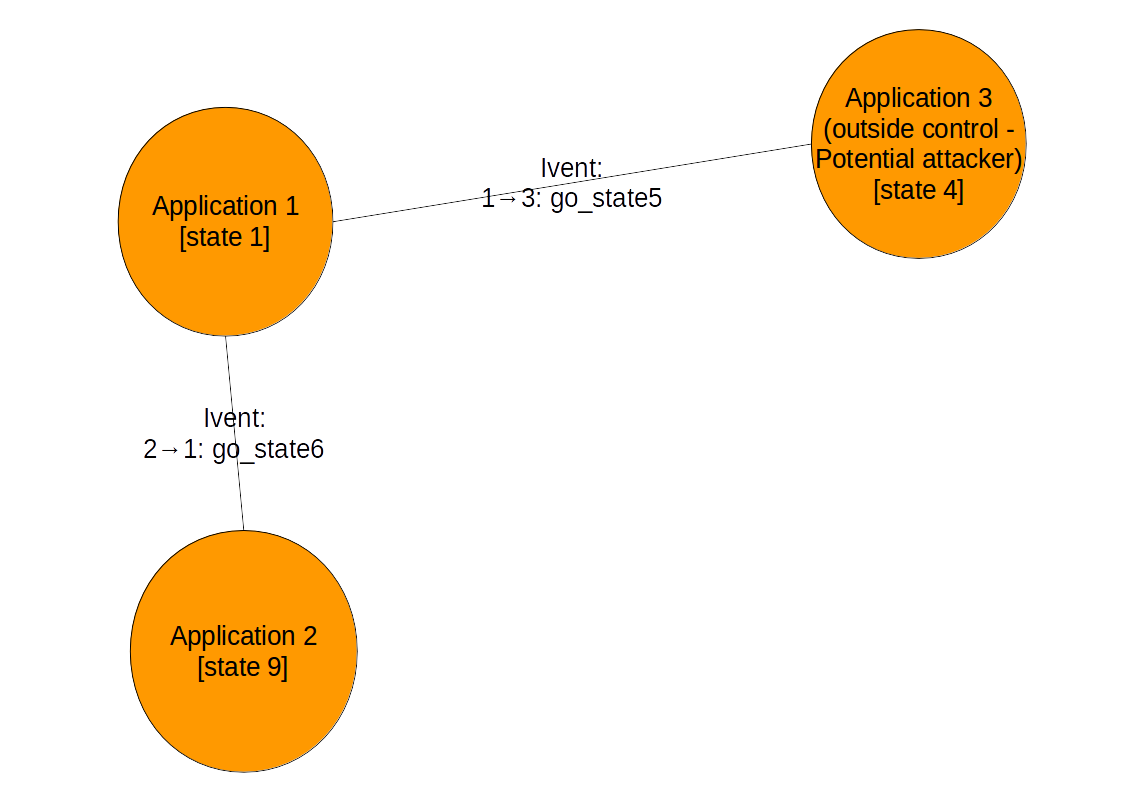
\includegraphics[width=\textwidth]{model}
    \caption{Aim of the project}
  \end{figure}
\end{frame}

\subsection{Technical choices}
\begin{frame}
  \frametitle{Technical choices: probes}
  \begin{figure}[h]
    \centering
    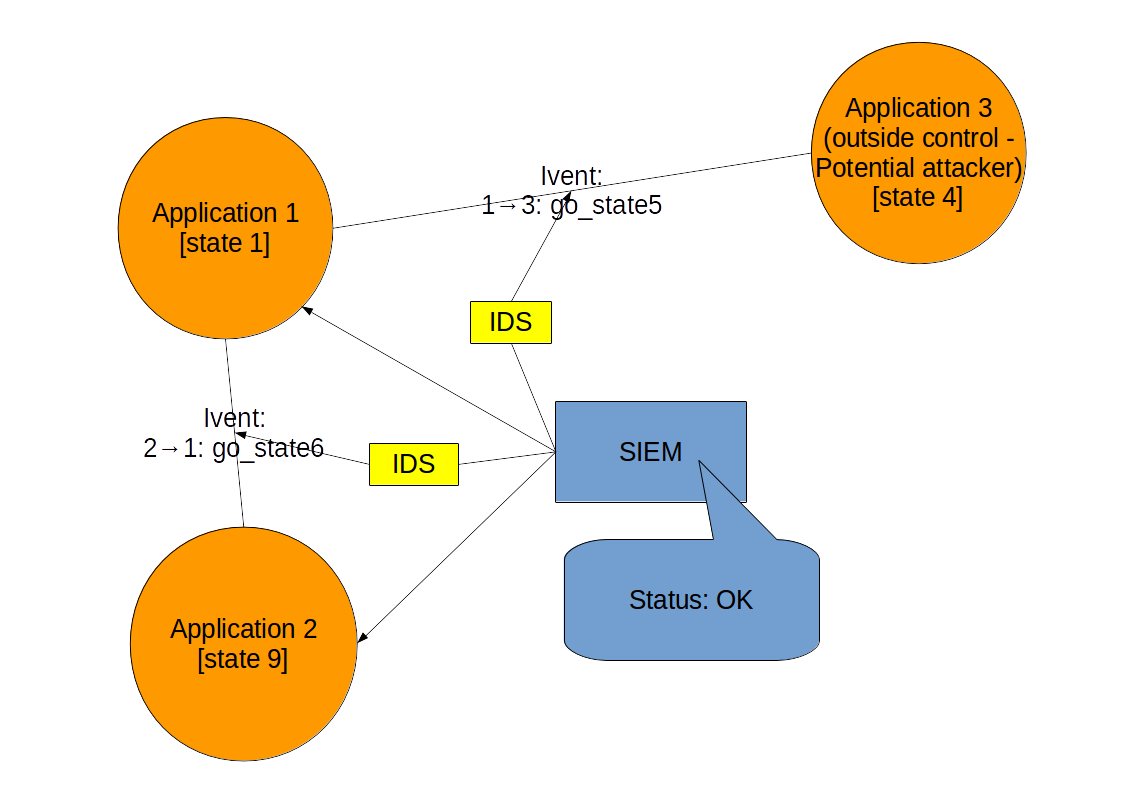
\includegraphics[width=\textwidth]{model_project}
    \caption{Aim of the project}
  \end{figure}
\end{frame}



\begin{frame}
  \frametitle{Technical choices: field of study}
  \begin{figure}[h]
    \centering
    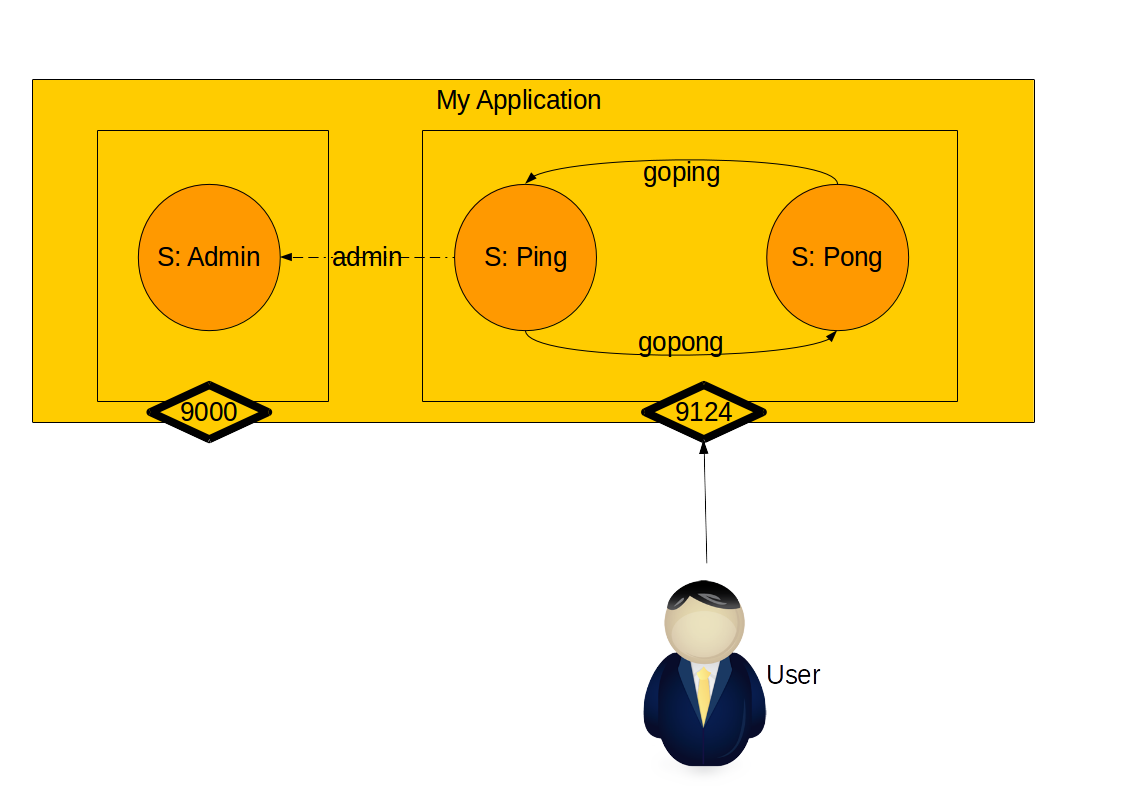
\includegraphics[width=\textwidth]{appli}
    \caption{Model of the application}
    \label{fig:model}
  \end{figure}
\end{frame}

\subsection{Organization}
\begin{frame}
  \frametitle{Organization}
  \begin{minipage}[h]{0.45\linewidth}
    \begin{figure}[h]
      \centering
      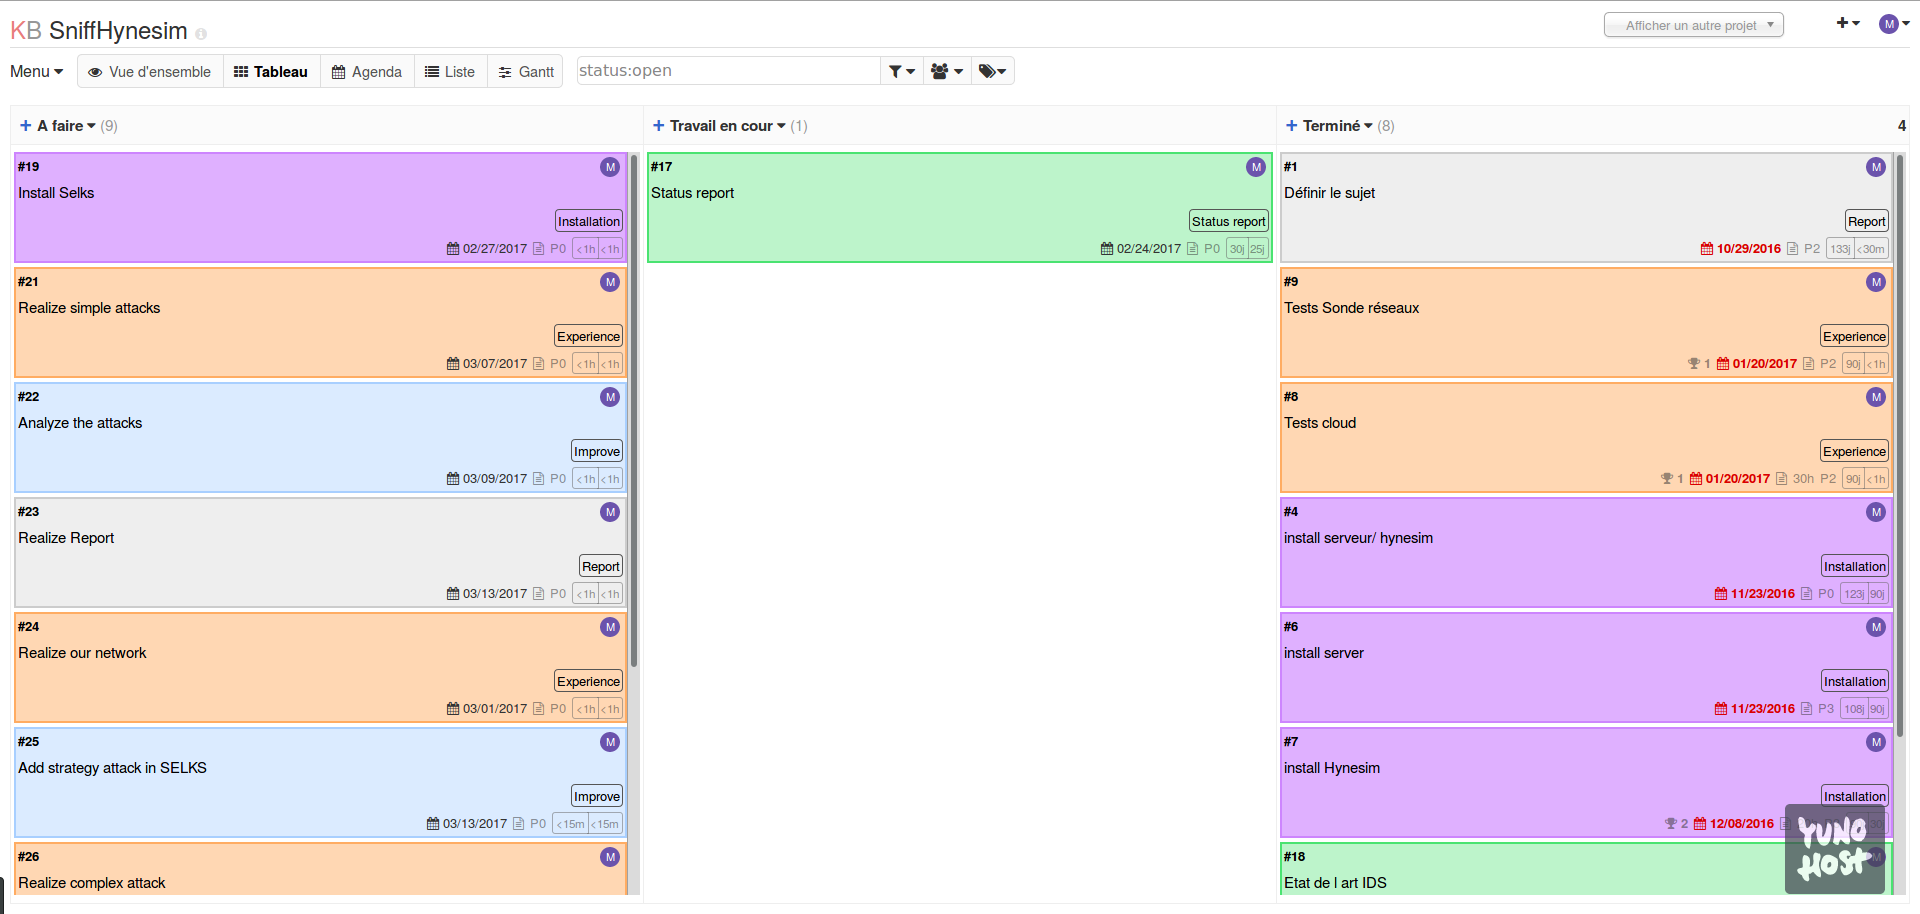
\includegraphics[width=1.2\textwidth]{kandboard}
      \caption{Kanban}
    \end{figure}
  \end{minipage}\hfill
  \begin{minipage}[h]{0.45\linewidth}
    \begin{figure}[h]
      \centering
      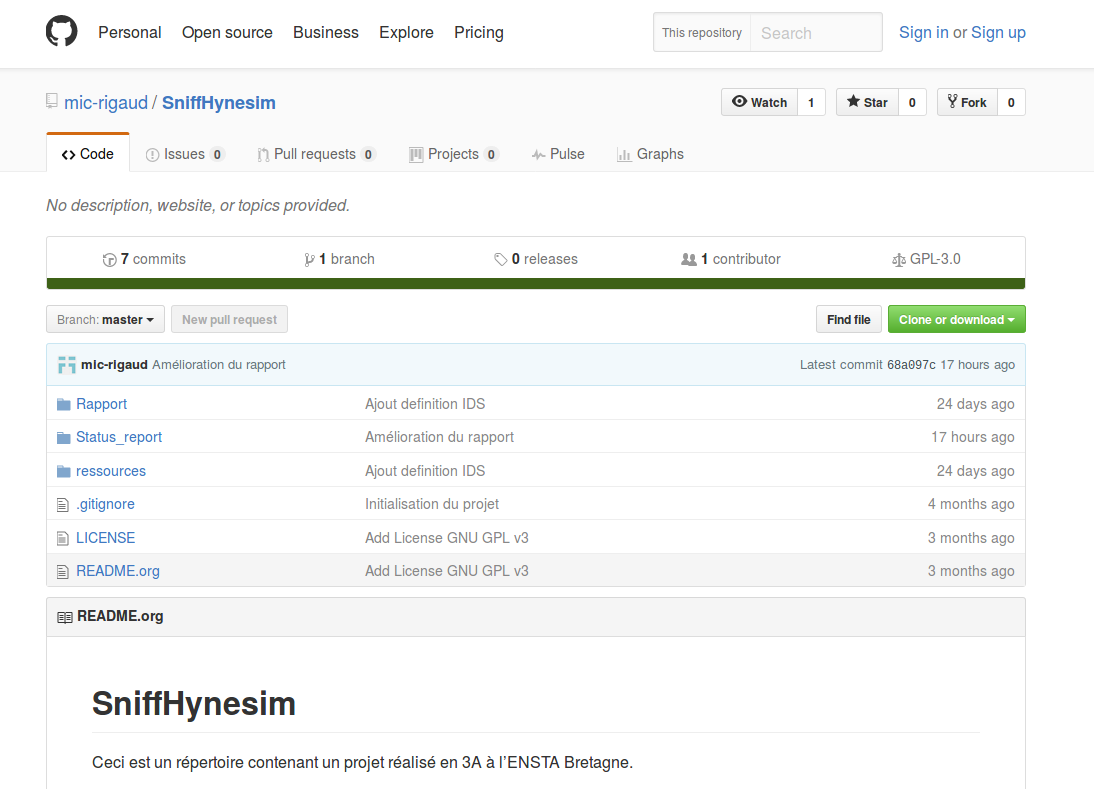
\includegraphics[width=0.8\textwidth]{github}
      \caption{Github}
    \end{figure}
  \end{minipage}
\end{frame}

%%%%%%%%%%%%%%%%%%%%%%%%%%%%%%%%%%%%%%%%%%%%%%%%%%%%%%%%%%%%%%%%%%%%%%%%%%%%%%%%%%%%%%%%%%%%%%%%%%%%%%%%%%%%%%
\section{Technical contribution}

\subsection{Installation}
\begin{frame}
  \frametitle{Installation}
  \begin{figure}[h]
    \centering
    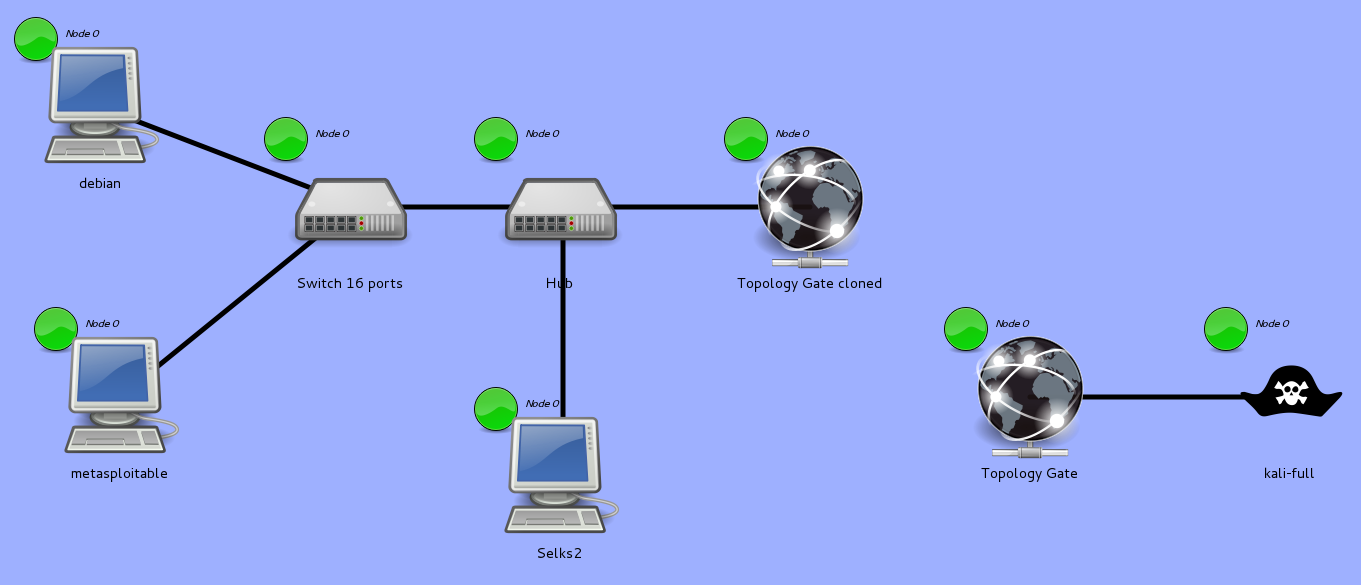
\includegraphics[width=\textwidth]{network_infra}
    \caption{Network installed}
  \end{figure}
\end{frame}

\subsection{Application}
\begin{frame}
  \frametitle{Application}

\end{frame}

\subsection{IDS}
\begin{frame}
  \frametitle{IDS}

\end{frame}

\subsection{SIEM}
\begin{frame}
  \frametitle{SIEM: Application probe}
  \begin{figure}[h]
    \centering
    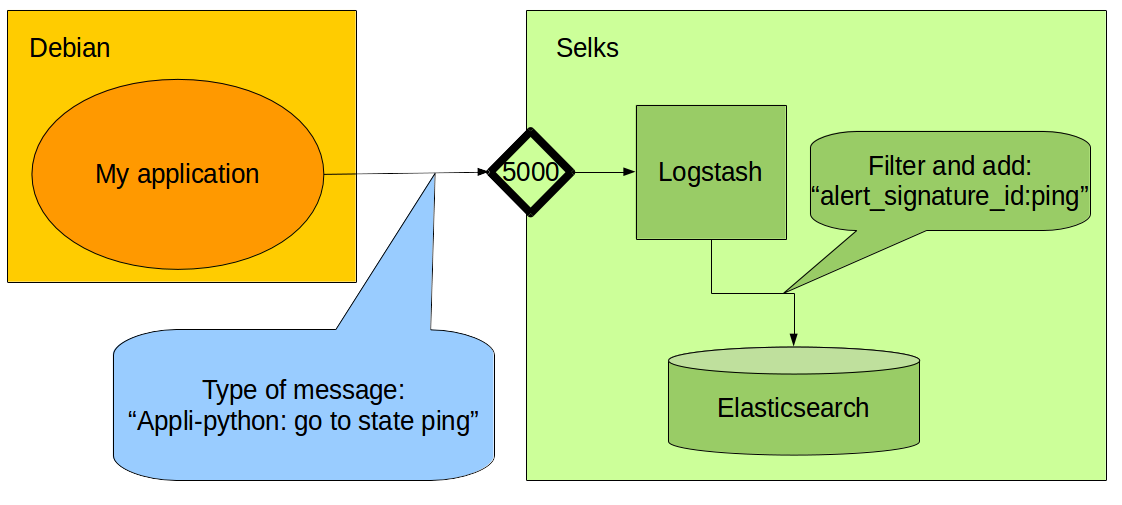
\includegraphics[width=\textwidth]{traitement_donnes}
    \caption{Data processing}
    \label{fig:data}
  \end{figure}
\end{frame}

\begin{frame}
  \frametitle{SIEM: Implementation}
  \begin{figure}[h]
    \centering
    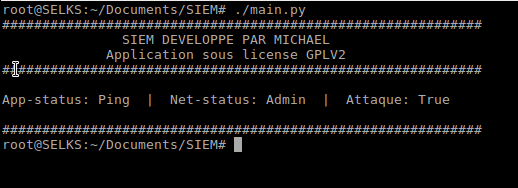
\includegraphics[width=\textwidth]{siem_interface}
    \caption{My SIEM}
  \end{figure}
\end{frame}

%%%%%%%%%%%%%%%%%%%%%%%%%%%%%%%%%%%%%%%%%%%%%%%%%%%%%%%%%%%%%%%%%%%%%%%%%%%%%%%%%%%%%%%%%%%%%%%%%%%%%%%%%%%%%%
\section{Results}

\subsection{Detection system}
\begin{frame}
  \frametitle{Detection system}
  \begin{figure}[h]
    \centering
    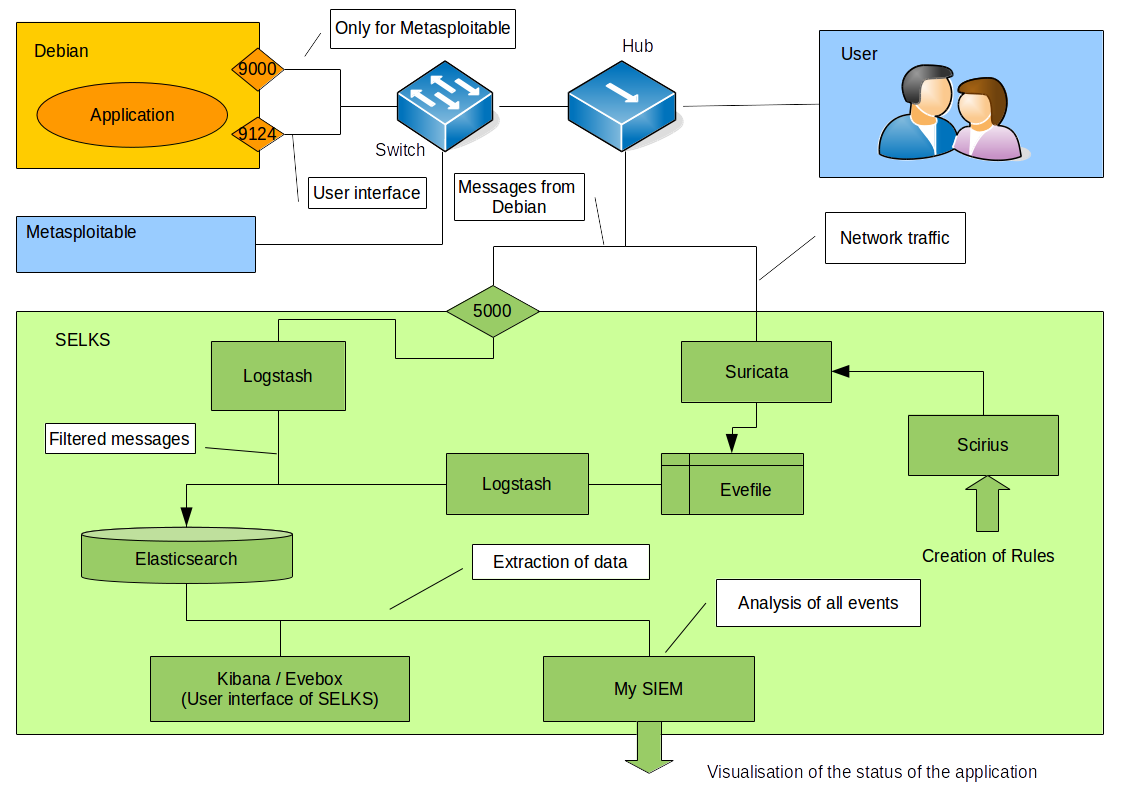
\includegraphics[width=\textwidth]{summary}
    \caption{Summary of the situation}
  \end{figure}
\end{frame}


\subsection{Results}
\begin{frame}
  \frametitle{Results}

\end{frame}

\subsection{Way of improvements}
\begin{frame}
  \frametitle{Way of improvements}

\end{frame}

%%%%%%%%%%%%%%%%%%%%%%%%%%%%%%%%%%%%%%%%%%%%%%%%%%%%%%%%%%%%%%%%%%%%%%%%%%%%%%%%%%%%%%%%%%%%%%%%%%%%%%%%%%%%%%
\section{Conclusion}
\begin{frame}
  \frametitle{Conclusion}

  \transdissolve[duration=0.1]
\end{frame}


\begin{frame}[allowframebreaks]
  \frametitle{Bibliography}
  \nocite{*}
  \bibliography{biblio}
  \transdissolve[duration=0.1]
\end{frame}


\begin{frame}
  \frametitle{Questions?}

  \begin{center}
    
\includegraphics[width=0.7\textwidth]{tux_ask}
  \end{center}
  \transdissolve[duration=0.1]
\end{frame}
\end{document}

%%% Local Variables:
%%% mode: latex
%%% TeX-master: t
%%% End:
